\documentclass[twoside,twocolumn,10pt]{article}

% -----------------------------
% Packages
% -----------------------------
\usepackage{fancyhdr}
\usepackage{geometry}
\usepackage{abstract}
\usepackage{graphicx}
\usepackage{titlesec}
\usepackage{ragged2e}
\usepackage{amssymb}
\usepackage{parskip}
\usepackage{amsmath}
\usepackage{newtxtext}
\usepackage{booktabs}
\usepackage{array}
\usepackage{balance}
\usepackage{xurl}
\usepackage{hyperref}
\usepackage[backend=bibtex,style=ieee]{biblatex}
\addbibresource{references.bib}
\usepackage[font=footnotesize,labelfont=bf,justification=raggedright,format=plain]{caption}
\usepackage{float}

% -----------------------------
% Bibliography Heading
% -----------------------------
\defbibheading{bibliography}[\refname]{%
  \section{\MakeUppercase{REFERENCES}}}

% -----------------------------
% Custom Column Types
% -----------------------------
\newcolumntype{L}[1]{>{\raggedright\arraybackslash}p{#1}}
\newcolumntype{C}[1]{>{\centering\arraybackslash}p{#1}}
\newcolumntype{R}[1]{>{\raggedleft\arraybackslash}p{#1}}

% -----------------------------
% Caption Formatting
% -----------------------------
\captionsetup[table]{labelsep=period, justification=raggedright}
\captionsetup[figure]{labelsep=period, justification=raggedright}

% -----------------------------
% Page Geometry
% -----------------------------
\geometry{
    a4paper,
    left=0.8in,
    right=0.8in,
    top=1in,
    bottom=1in
}

\setlength{\columnsep}{15pt}
\setlength{\parindent}{0pt}
\setlength{\parskip}{0pt}
\hyphenpenalty=10000
\exhyphenpenalty=10000
\frenchspacing

% -----------------------------
% Abstract Formatting
% -----------------------------
\renewcommand{\abstractname}{\hspace{1.3em}\textbf{Abstract}}
\renewcommand{\abstractnamefont}{\normalfont\fontsize{10}{14}\bfseries\MakeUppercase}
\renewcommand{\absnamepos}{flushleft}
\renewcommand{\abstracttextfont}{\normalfont\fontsize{11}{13}\selectfont}

% -----------------------------
% Header / Footer Style
% -----------------------------
\setcounter{page}{1}
\pagestyle{fancy}
\fancyhf{}
\fancyhead[C]{\small SHORT PAPER TITLE}
\fancyhead[CO]{\small Raquel Castro (2026)}
\fancyfoot[C]{\thepage}

% -----------------------------
% First Page Style
% -----------------------------
\fancypagestyle{firstpage}{
  \fancyhf{}
  \fancyhead[LO]{\small Volume X, Issue X, Year}
 \fancyhead[RO]{\small LGU J. Comput. Sci. \& IT}
  \fancyfoot[L]{\footnotesize Received: DD Month YYYY; Revised: DD Month YYYY; Accepted: DD Month YYYY\\\textsuperscript{*}Corresponding Author: Name \textless email@example.com\textgreater}
  \fancyfoot[R]{\footnotesize \textcopyright\ Year by the Author(s). Published by LGURJCSIT,\\ \hspace{0.5cm} under the CC-BY license}
  \renewcommand{\headrulewidth}{0.4pt}
  \renewcommand{\footrulewidth}{0.4pt}
}

% -----------------------------
% Title / Author
% -----------------------------
\title{\fontsize{16}{20}\selectfont\textbf{Predicting Inflammatory Bowel Disease Using Gut Microbiome Profiles}}

\author{
    \fontsize{12}{14}\selectfont
    Raquel Castro\textsuperscript{1}\\[1ex]
    \fontsize{12}{14}\selectfont
    \textsuperscript{1}Faculdade de Ciências da Universidade do Porto \\
}

\date{}

% -----------------------------
% Section Formatting
% -----------------------------
\titleformat{\section}{\normalsize\bfseries\uppercase}{\thesection.}{1em}{}
\titleformat{\subsection}{\normalsize\bfseries\flushleft}{\thesubsection.}{1em}{}
\titleformat{\subsubsection}{\normalsize\bfseries\itshape\flushleft}{\thesubsubsection.}{1em}{}

% -----------------------------
% Document Start
% -----------------------------
\begin{document}

\twocolumn[
\begin{@twocolumnfalse}

\vspace{-0.7cm}
\noindent
\raggedright
{\fontsize{11}{13}\selectfont Original Article}
\hfill
{\fontsize{11}{13}\selectfont\footnotesize https://doi.org/xx.xxxx/xxxx}

\vspace{-0.5cm}

\maketitle
\thispagestyle{firstpage}

\section*{\hspace{-1.5mm}Abstract}
\fontsize{10}{12}\selectfont
\justifying
\noindent
Inflammatory bowel disease (IBD) is associated with alterations in the gut microbiome, making microbial profiles a promising source of diagnostic biomarkers. In this study, gut microbiome data were preprocessed using prevalence filtering and centered log-ratio (CLR) transformation before training five supervised machine learning models. Model performance was evaluated using repeated nested group-stratified cross-validation, with the Random Forest classifier achieving the best performance (ROC AUC = 0.707) on an independent test set. SHAP analysis identified bacterial taxa influencing the model predictions, many of which have previously been associated with IBD. These findings demonstrate the potential of explainable machine learning for microbiome-based disease prediction and biomarker discovery.


\vspace{0.8cm}
\end{@twocolumnfalse}
]

% -----------------------------
% Main Text
% -----------------------------
\section{Introduction}
\fontsize{11}{13}\selectfont

Inflammatory bowel disease (IBD) is characterized as a chronic disease of inflammatory nature that comprises Crohn's disease (CD) and Ulcerative Colitis (UC) (Khor, \textit{et al.}, 2011). Ulcerative colitis is strictly limited to the colon and rectum with a continuous pattern of mucosal inflammation. Chron’s Disease can appear anywhere from mouth to anus and is characterized by patches of transmural inflammation (Xavier, \textit{et al.}, 2007). It has previously been proposed that the epidemiology of IBD evolves predictably across four distinct epidemiological stages determined by changes in incidence and prevalence. The four stages are: 1) emergence; 2) acceleration in incidence; 3) compounding prevalence and 4) prevalence equilibrium (Hindson, 2025). The incidence and prevalence of IBD in western countries have increased sharply in the 20th century, and continues to increase (Kaplan, 2025; Lee, \textit{et al.}, 2023). The International Organization for the Study of Inflammatory Bowel Disease (IOIBD) estimates that in these countries more than 20 out of 100 000 people live with stage 4 of the disease. Early and newly industrialized countries are expected to shift from stage 3 to 4 in the next decade (Kaplan, 2025). Given the growing prevalence of the late stages of the disease, identifying potential molecular targets for prediction and or therapeutic intervention has become more important than ever. Such advances could significantly improve the quality of life of the patients affected by IBD and alleviate the burden on the healthcare system. The central issue with IBD is that its etiology remains unknown. Current evidence indicates that environmental exposures, dietary patterns, alterations in the commensal microbiota, genetic susceptibility, or a combination of these factors contribute to disease onset and progression (Pereira, \textit{et al.}, 2024). The role of the gut microbiota in IBD, whether as a potential therapeutic target or as a diagnostic biomarker, has become an increasingly prominent focus within the research community. A simple search in Scopus using the terms “IBD” and “microbiota” illustrates this trend: the number of publications has expanded approximately 107‑fold over the past two decades, rising from 27 articles in 2006 to 2900 in 2025. In fact, dysbiosis of the gut microbiota is characterized by alterations in the ratio of pro-inflammatory and anti-inflammatory microorganisms (Zhao et al., 2023). Given the size of the population of bacteria that live inside our gut, that even prompted the “our second genome” name, and their immunomodulatory capabilities, it is easy to understand the rise in interest of the research community on this topic (Grice et al., 2012; Chen et al., 2025). Approximately, 98\% of intestinal bacteria belong to four major bacterial phyla, namely, Bacteroidetes, Firmicutes, Proteobacteria, and Actinobacteriota. It appears that the genera Bacteroides, Clostridium, Lactobacillus, Enterobacteriaceae, and Bifidobacterium from the four major bacterial phyla play an important role in the regulation of chronic intestinal inflammation (Ananthakrishnan, \textit{et }al., 2018; Chen et al., 2025; Wang, \textit{et al.}, 2026;  Schirmer, \textit{et al., 2019). }

Several studies over the years have tried to characterize the composition and diversity of the human microbiome: The Human Microbiome project (2007-2014), Metagenomics of the Human Intestinal Tract (2008-2012), The Global Microbiome Conservancy (2016-ongoing). The American Gut Project (2012-ongoing with the Microsetta Initiative). These studies established multiple datasets of human microbial communities with extensive amounts of data, which holds great promise for discovering subtle microbial population patterns and heterogeneities that are impossible with small-scale data. On the other hand, the massive sample size and high dimensionality of large amounts of data introduce unique computational and statistical challenges. These challenges are distinguished and require new computational and statistical paradigms (Fan et al., 2014). Enters the era of Artificial Intelligence (AI). Machine learning (ML) is a subset of AI that is able to handle large amounts of data to recognize, classify and predict patterns. Owing to its powerful informative and predictive potential, ML  and deep learning are evolving as important tools to advance microbiome research (Hérnandez Medina et al., 2022). The aim of this study was to investigate whether a machine learning model could accurately predict the diagnostic outcome of individuals based solely on their gut microbiome composition. Specifically, to distinguish between individuals diagnosed with IBD, including CD and UC, and generally healthy participants. To achieve this, a publicly available dataset containing bacterial species abundance data from healthy individuals, CD patients, and UC patients was analyzed. Several machine learning models were trained and evaluated, with each model undergoing hyperparameter optimization to maximize predictive performance. The models were then compared to identify the approach that achieved the highest classification accuracy while highlighting the bacterial species that contributed most to the predictions.


\section{Methodology}
\fontsize{11}{13}\selectfont

\subsection{Data Preparation}
The data is a curated, Machine Learning-ready version of the Integrative Human Microbiome Project (iHMP), specifically the Inflammatory Bowel Disease Multi-omics Database (IBDMDB), available on kaggle (Qasim Hussain. 2026). Figure 1 provides a schematic representation of the methodologies employed in the study. The data corresponds to a cohort of 3387 longitudinal stool metagenomes from 130 participants, distributed over three groups, Healthy, Crohn’s Disease and Ulcerative Colitis, followed across 52 weeks. Features include the Participants ID, number of weeks being followed up to date, diagnosis, levels of faecal calprotectin and the abundance profile of 566 different species of bacteria. The dataset was used to train and evaluate multiple machine learning models. Each model was optimized using different hyperparameter configurations, and their predictive performance was compared to identify the model that most accurately classified the outcome based on the most informative bacterial species. As a preprocessing step, only bacterial species present in more than 10\% of the participants were retained to reduce data sparsity. The filtered abundance data were subsequently transformed using the centered log-ratio (CLR) transformation to account for the compositional nature of microbiome data. The CLR-transformed values were then used as input features to train and evaluate the models. The dataset was divided into training (70\%) and testing (30\%) subsets using GroupShuffleSplit. Grouping by participant ID ensured that all samples from a given participant were assigned to a single subset, preventing overlap between the training and testing data and reducing the risk of data leakage.  

\subsection{Model Building}
For the binary classification task, participants diagnosed with Crohn's disease or ulcerative colitis were grouped into a single IBD class, whereas healthy participants constituted the Healthy class. Model selection and performance evaluation were conducted using repeated nested group-stratified cross-validation (Figure 2). Five models were tested: Decision Tree, Random Forest, Extra Tree, Gradient Boosting and XGBoost. The outer cross-validation procedure consisted of five folds and was used to estimate model generalization performance. Within each outer training fold, a four-fold inner cross-validation procedure was used to optimize model hyperparameters through an exhaustive grid search. Hyperparameter selection was based on the mean area under the receiver operating characteristic curve (ROC AUC) obtained across the inner folds. Both the inner and outer cross-validation procedures were implemented using stratified group-based splitting. Participant ID was used as the grouping variable to ensure that all samples from the same participant were assigned to only one fold. Stratification was applied to preserve the class distribution as closely as possible across folds. Following hyperparameter optimization, the model with the best inner cross-validation score was refitted using the complete outer training set and evaluated on the corresponding outer validation set. Performance was assessed using accuracy, precision, sensitivity, specificity, F1 score, and ROC AUC. The nested cross-validation procedure was repeated three times using different random seeds, resulting in 15 outer validation evaluations per model. The optimal hyperparameters selected for each outer fold were also recorded. The best model was subsequently evaluated on the independent test set comprising previously unseen data. The resulting performance metrics were compared with those obtained during the cross-validation stage to assess the model's generalization ability. Finally, a confusion matrix was generated to visualize the model's classification performance. 

\subsection{Feature Selection}
To improve interpretability, feature importance was assessed using SHapley Additive exPlanations (SHAP). SHAP works by quantifying the contribution of each feature to an individual prediction, thereby providing both local and global model interpretability. SHAP values were calculated using the TreeExplainer algorithm. The trained model was applied to the independent test set, and SHAP values were computed for all features. For binary classification, the SHAP values corresponding to the positive class (IBD) were used to assess feature importance. Global feature importance was visualized using a SHAP beeswarm plot. The twenty most influential features were displayed in the final visualization. The bacterial features identified as most influential by the final machine learning model were further evaluated for differences between the diagnostic groups. For each selected bacterial feature, the distributions of the centered log-ratio-transformed values were compared between participants with IBD and Healthy participants using a two-sided Mann-Whitney U test. This non-parametric test was used to assess whether the feature distributions differed between the two diagnostic groups. To account for multiple hypothesis testing, the resulting p-values were adjusted using the Benjamini-Hochberg false discovery rate procedure. Features with an adjusted p-value below 0.05 were considered statistically significant. Statistically significant features were visualized using boxplots, summarizing the distributions of each bacterial feature within the Healthy and IBD groups. 

% -----------------------------
% Figure 1
% -----------------------------
\begin{figure*}[t]
\centering
\includegraphics[width=0.82\textwidth]{Captura de ecrã 2026-07-29 215429.png}
\caption{\textbf{Schematic representation of the methodology employed in this study.} The workflow comprises three sequential phases: data preparation, including dataset collection, preprocessing (prevalence filtering, CLR transformation and data partitioning); model building, including hyperparameter optimization using nested cross-validation, model training, and validation; and feature selection, in which SHAP was used to quantify feature importance, followed by statistical comparison of the most influential bacterial species between Healthy individuals and patients with IBD using the Mann-Whitney U test with Benjamini-Hochberg false discovery rate correction. Adapted from BioRender.}
\label{figure1}
\end{figure*}

% -----------------------------
% Figure 2
% -----------------------------
\begin{figure*}[t]
\centering
\includegraphics[width=0.82\textwidth]{Captura de ecrã 2026-07-29 222442.png}
\caption{\textbf{Illustration of the nested group-stratified cross-validation framework employed for model development.} The outer loop estimates the generalization performance of the model by repeatedly partitioning the data into training and validation folds. Within each outer training fold, an inner group-stratified cross-validation procedure is used to optimize model hyperparameters through grid search. The optimal hyperparameters are then used to retrain the model on the complete outer training data before evaluation on the corresponding outer test set fold. Created with BioRender.}
\label{figure2}
\end{figure*}

\section{Results}
\fontsize{11}{13}\selectfont

\subsection{Data Analysis}
The dataset comprised 3,387 observations and 571 features, including an External ID, Participant ID, the week following enrollment, the diagnosis (Healthy, Crohn's disease, or Ulcerative Colitis), fecal calprotectin levels ($\mu$/g), and the abundance profiles of 566 bacterial species (Figure 3). 

The fecal calprotectin is an established marker of gut inflammation in IBD, serving as a diagnostic and therapeutic marker of inflammatory disease activity. For healthy individuals the values of calprotectin typically range from 10 to 50 $\mu$g per g of stool, whereas in acute inflammation it can increase by up to 10 fold to more than 600 $\mu$/g. The threshold for IBD diagnosis usually happens above 100-200 $\mu$g/g (Heinzel et al., 2024). In this dataset the measurements of fecal calprotectin are missing in 2027 entries, corresponding to 59.8\% of all entries. The initial objective of this project was to evaluate the predictive performance of microbiome data in comparison with fecal calprotectin levels. To address the missing data, several imputation strategies were explored, including median imputation and k-nearest neighbors (KNN) imputation. However, given the substantial proportion of missing values, these approaches were considered unlikely to produce reliable estimates and risked introducing significant bias into subsequent analyses. Consequently, the fecal calprotectin variable was excluded from the final dataset, and the study focused exclusively on the microbiome for predictive modeling.


One of the main challenges of this dataset was its high degree of sparsity. A total of 269 bacterial species were absent (zero abundance) in at least 99\% of the samples, while 531 species were absent in at least 50\% of the samples. Such a high proportion of zero values can adversely affect machine learning performance by increasing data sparsity and introducing noise into the modeling process. To reduce the dimensionality of the dataset and mitigate the effects of sparsity, a prevalence filter was applied. Only bacterial species present in at least 10\% of the participants were retained for subsequent analyses (Figure 4). This preprocessing step removed 440 bacterial species, leaving 126, resulting in a more informative feature set for model training.

% -----------------------------
% Figure 3
% -----------------------------
\begin{figure}[t]
    \centering
    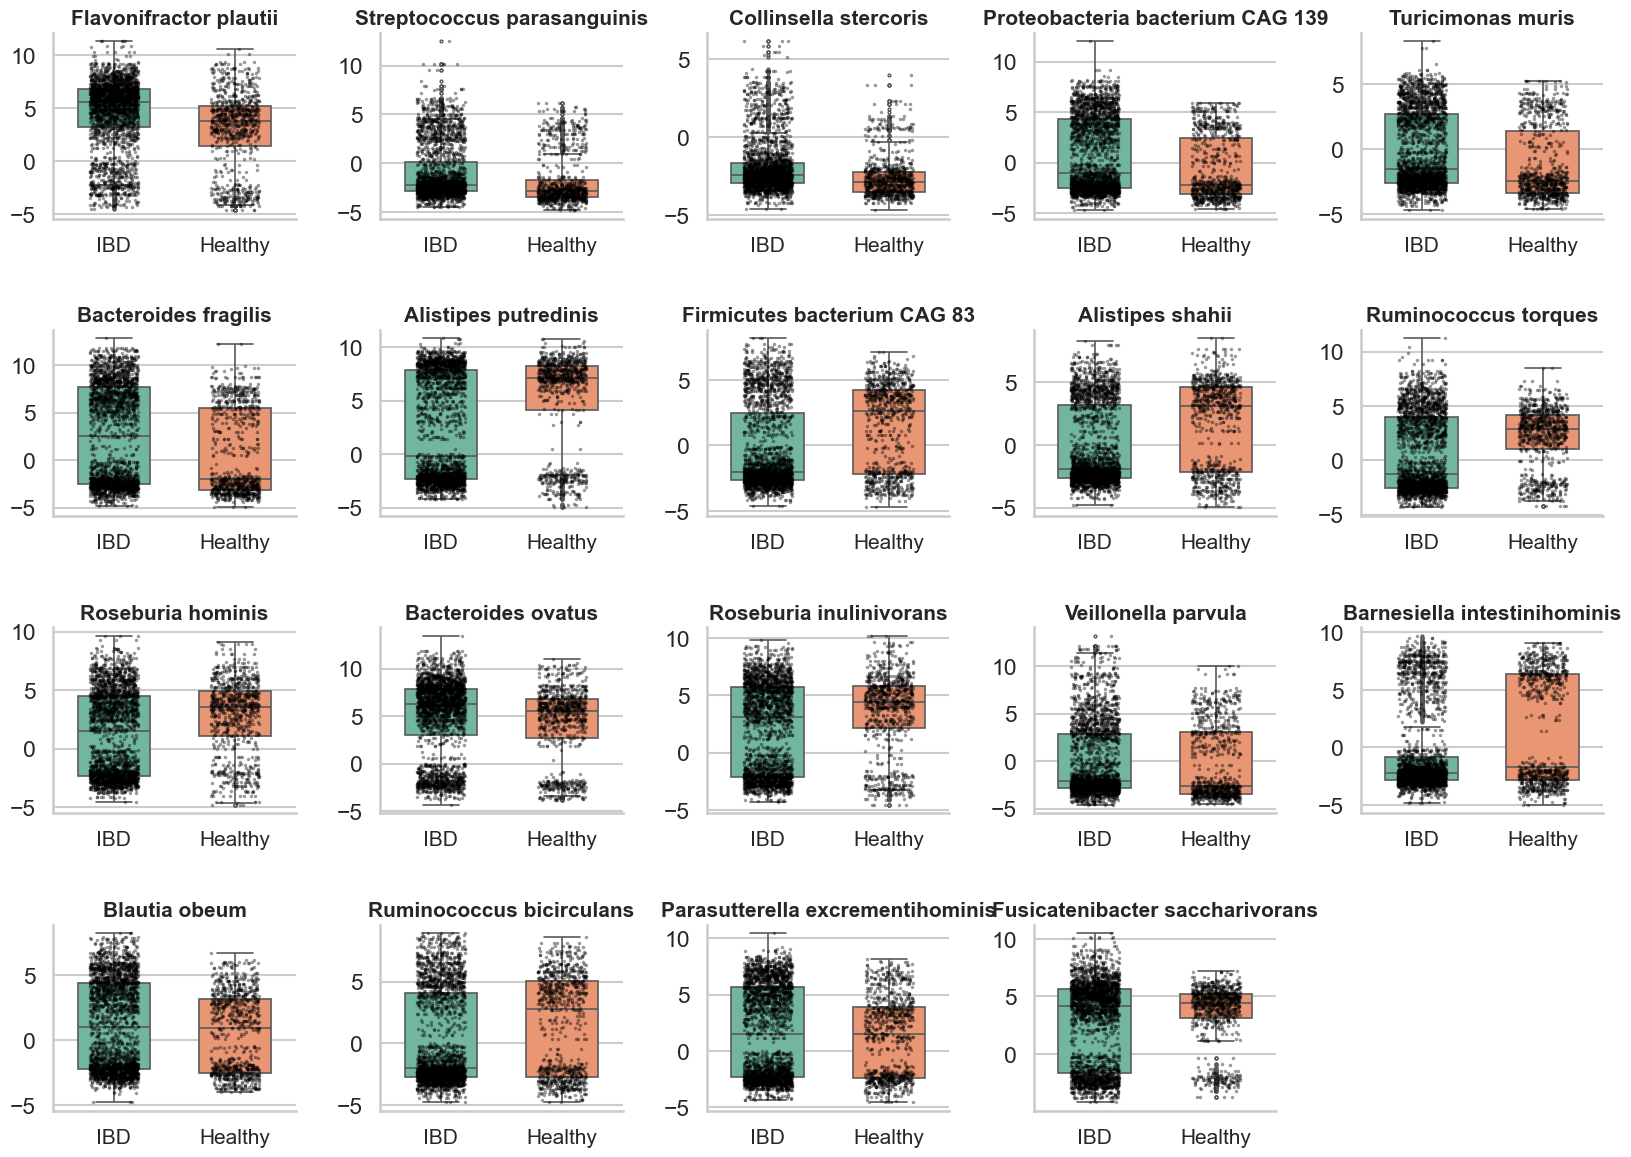
\includegraphics[width=0.3\textwidth]{output.png}
    \caption{\textbf{Distribution of diagnostic categories among the study participants.} A total of 116 patients were included in the study. The figure shows the percentage of patients in each diagnostic group. Crohn’s disease represented the largest proportion of the cohort, accounting for 47.476\% of participants, followed by ulcerative colitis at 26.956\%. Healthy individuals comprised the remaining 25.568\% of participants.}
    \label{Figure3}
\end{figure}

% -----------------------------
% Figure 4
% -----------------------------
\begin{figure}[t]
    \centering
    \includegraphics[width=0.3\textwidth]{prevalence.png}
    \caption{\textbf{Histogram of bacterial species prevalence across the study cohort.} Prevalence was calculated as the proportion of participants in which each bacterial species was detected. The distribution demonstrates that most species were detected in only a small fraction of participants, highlighting the sparse nature of the microbiome dataset.}
    \label{Figure4}
\end{figure}

\subsection{Model Assessment}
As mentioned above, the predictive performance of the machine learning algorithms was evaluated by a repeated nested grouped cross-validation. The outer loop consisted of five stratified grouped folds and was repeated three times, resulting in fifteen independent evaluations for each model. Hyperparameter optimization was performed within the inner four-fold stratified grouped cross-validation using ROC AUC as the optimization metric. Grouping by participant ensured that samples from the same individual were never simultaneously included in both the training and validation sets, preventing data leakage. Table 1 summarizes the results more clearly.

One of the things that stands out is how ensembles consistently outperformed the Decision Tree classifier (Table 1). In fact, Decision Tree achieved the lowest results for almost all evaluation metrics. A ROC AUC value of \(0.501 \pm 0.133\) indicates a predictive power close to random. Of all the ensembles, Random Forest exhibited the strongest overall performance, achieving the highest ROC AUC (0.625 ± 0.130) and F1 score (0.857 ± 0.021), together with a high accuracy (0.766 ± 0.034). Extra Trees produced the highest mean accuracy (0.746 ± 0.054), while XGBoost achieved the highest recall (0.938 ± 0.052), indicating superior sensitivity for identifying IBD cases. Gradient Boosting showed comparable performance, with an F1-score of 0.842 ± 0.028 and a recall of 0.911 ± 0.046. Given the highest ROC AUC results, Random Forest was crowned the best model, specifically the hyperparameters \{max\_depth: 5, max\_features: log2, min\_samples\_leaf: 2, min\_samples\_split: 2, n\_estimators: 500\}.
One thing to note is that although precision remained very similar across all ensemble models, specificity was always significantly lower than recall, ranging from 0.133-0.338 to the first vs 0.867-0.938 to the latter. This means that although the model correctly diagnosed most of the positive cases, IBD, it incorrectly diagnosed a big proportion of the negative cases. This points to the class imbalances previously described, with more IBD participants compared to healthy.

% -----------------------------
% Table 1
% -----------------------------
\begin{table*}[t]
\centering
\caption{\textbf{Average performance of each classifier across all outer validation folds.} Performance is reported as the mean and standard deviation of Accuracy, Precision, Recall, Specificity, F1-score, and ROC AUC.}
\label{tab:classifier_performance}

\resizebox{\textwidth}{!}{%
\begin{tabular}{lcccccccccccc}
\toprule
& \multicolumn{2}{c}{Accuracy} &
\multicolumn{2}{c}{Precision} &
\multicolumn{2}{c}{Recall} &
\multicolumn{2}{c}{Specificity} &
\multicolumn{2}{c}{F1-score} &
\multicolumn{2}{c}{ROC AUC} \\
\cmidrule(lr){2-3}
\cmidrule(lr){4-5}
\cmidrule(lr){6-7}
\cmidrule(lr){8-9}
\cmidrule(lr){10-11}
\cmidrule(lr){12-13}
Model &
Mean & Std &
Mean & Std &
Mean & Std &
Mean & Std &
Mean & Std &
Mean & Std \\
\midrule
Decision Tree &
0.601888 & 0.112477 &
0.776922 & 0.065969 &
0.678108 & 0.156713 &
0.341386 & 0.207783 &
0.715375 & 0.112284 &
0.501476 & 0.133169 \\

Extra Trees &
0.746390 & 0.054224 &
0.817909 & 0.035166 &
0.867243 & 0.071299 &
0.337960 & 0.170836 &
0.840023 & 0.037457 &
0.610052 & 0.143101 \\

Gradient Boosting &
0.737359 & 0.042645 &
0.784052 & 0.024504 &
0.911365 & 0.045710 &
0.145651 & 0.117557 &
0.842429 & 0.027766 &
0.566437 & 0.122061 \\

Random Forest &
0.765924 & 0.034285 &
0.812497 & 0.028186 &
0.908582 & 0.041072 &
0.280953 & 0.154515 &
0.857014 & 0.020658 &
0.624650 & 0.129637 \\

XGBoost &
0.755139 & 0.034324 &
0.786910 & 0.022786 &
0.938486 & 0.051877 &
0.133159 & 0.129309 &
0.855089 & 0.023319 &
0.565863 & 0.103164 \\
\bottomrule
\end{tabular}
}
\end{table*}

\subsection{Predictive Power}
Following the results obtained in the nested cross-validation its predictive performance was assessed on the untouched test set. Again the same performance metrics were calculated, Accuracy, Precision, Recall, Specificity, F1 score and ROC AUC. The results obtained on the independent test set vs the ones obtained during cross-validation are presented in Table 2. Comparing these values with those obtained during nested cross-validation allowed the assessment of whether the selected model generalized well to previously unseen data or exhibited signs of overfitting.
From Table 2 we can see that the test set performance is very similar to the nested cross validation performance, this indicates that the model made reasonably well generalisations to the unseen data. The model achieved an accuracy of 0.740, compared with a mean cross validation accuracy of 0.766. Precision decreased slightly from 0.812 during cross validation to 0.739 on the test set, while recall increased from 0.909 to 0.943, indicating that the model maintained a high sensitivity for correctly identifying participants with IBD. Similarly, the F1 score decreased only modestly from 0.857 to 0.829, suggesting that the balance between precision and recall remained stable. The ROC AUC increased from 0.625 during nested cross-validation to 0.707 on the test set, demonstrating a moderate improvement in the model's overall discriminative ability. Specificity, however, increased only slightly from 0.281 during cross validation to 0.333 on the independent test set; it consistently remained substantially lower than recall, indicating that the classifier was considerably more effective at identifying participants with IBD than healthy controls.
As shown in the confusion matrix (Figure 5), the model correctly predicted 567 out of 601 samples belonging to participants with IBD, compared to only a third of the samples belonging to healthy patients being correctly predicted. This once again points to the model having high sensitivity for identifying IBD samples but comparatively lower specificity for correctly classifying healthy participants.

% -----------------------------
% Table 2
% -----------------------------
\begin{table}[ht]
\centering
\caption{\textbf{Comparing model performance on the independent test set vs. nested cross-validation.} Performance of the selected Random Forest classifier during repeated nested cross-validation and on the independent test set, evaluated using accuracy, precision, recall, specificity, F1-score, and ROC AUC.}
\label{tab:rf_comparison}

\resizebox{\linewidth}{!}{%
\begin{tabular}{lcc}
\toprule
\textbf{Metric} & \textbf{Nested CV Mean} & \textbf{Final Test} \\
\midrule
Accuracy    & 0.765924 & 0.740289 \\
Precision   & 0.812497 & 0.739244 \\
Recall      & 0.908582 & 0.943428 \\
Specificity & 0.280953 & 0.333333 \\
F1-score    & 0.857014 & 0.828947 \\
ROC AUC     & 0.624650 & 0.707393 \\
\bottomrule
\end{tabular}
}
\end{table}

% -----------------------------
% Figure 5
% -----------------------------
\begin{figure}[ht]
    \centering
    \includegraphics[width=\linewidth]{confusion matrix.png}
    \caption{\textbf{Confusion matrix of the Random Forest classifier evaluated on the independent test set.} The matrix summarizes the number of correctly and incorrectly classified samples for the two outcome classes, Healthy and IBD. Rows represent the true class labels and columns represent the predicted class labels.}
    \label{Figure 5}
\end{figure}

\subsection{Feature Importance}
In order to infer which features were driving the model predictions, I conducted the SHAP method on the independent test set, which summarizes how the Random Forest model made its predictions on the unseen data (Figure 6). The graph can be interpreted as follows: Rows represent the 20 bacterial species with the highest absolute mean SHAP value; each dot in the row represents a single sample from a given participant; on the x-axis we can see the SHAP values that indicate how strongly that feature contributed to the models outcome- positive values push the prediction toward IBD prediction, whilst negative values push the prediction toward healthy prediction; the colour is an indicative of the CLR-transformed abundance of the bacteria, with the red colour indicating an increased abundance and blue colour indicating a decreased abundance.
From the graph we can see that different bacteria have different directional effects. Firmicutes bacterium CAG 83, Roseburia inulinivorans, Alistipes putredinis, Ruminococcus torques, Roseburia hominis have the highest SHAP values where decrease levels lead towards an IBD outcome. This suggests that higher levels of these bacteria are associated with the Healthy class, whereas lower levels increase the probability of IBD. On the other hand, some species exhibit the opposite relationship. Turicimonas muris, Proteobacteria bacterium CAG 139, Flavonifractor plauti, Blautia obeum, Parasutterella excrementihominis and Bacteroides fragilis are amongst the bacteria where higher abundance corresponds to positive SHAP values, indicating that increased abundance contributes toward predicting IBD. One important consideration is that most SHAP values lie close to zero, indicating that no single bacterial species seems to determine the prediction by itself. Instead, the Random Forest combines information from many bacterial species to generate the final classification. On the final row, “Sum of 107 other features” represents the combined contribution of all the other bacteria whose SHAP values alone were too low to be represented by themselves. But we can see that although each of these features alone have a very small effect on the model’s prediction, together they contribute substantially to the outcome of the prediction. This highlights that the classifier seems to rely on a broad microbial signature rather than a few dominant features.

% -----------------------------
% Figure 6
% -----------------------------
\begin{figure*}[t]
\centering
\includegraphics[width=0.82\textwidth]{SHAP_results.png}
\caption{\textbf{SHAP summary plot for the Random Forest classifier evaluated on the independent test set.} The bacterial species are ranked according to their mean absolute SHAP values, with higher-ranked species contributing more strongly to the model's predictions. Positive SHAP values indicate an increased probability of classification as inflammatory bowel disease (IBD), whereas negative values favor classification as healthy. In turn, the red and blue colours indicate if the feature driving the prediction comes from decreased (blue) or increased (red) levels of that feature, in this case the bacteria species. }
\label{figure6}
\end{figure*}

\subsection{Statistical Significance}
Next I wanted to analyze whether the bacteria identified as important by the model had statistically different levels of CLR-transformed abundance between healthy and IBD participants. For the statistical test, a non-parametric approach was deployed, the Mann-Whitney U test. Benjamini-Hochberg False Discovery rate was used to correct for multiple testing. The median CLR, for each bacteria in Healthy vs IBD setting along with p-value and adjusted p-value are presented in Table 3. Several bacteria have noticeably higher median CLR values in the IBD group compared to that of Healthy individuals. Flavonifractor plautii, Proteobacteria bacterium CAG 139, Turicimonas muris, Bacteroides fragilis, Streptococcus parasanguinis, Collinsella stercoris. Bacteroides fragilis, for example, has a median CLR abundance of approximately 2.51 in the IBD group compared with $-2.02$ in the Healthy group. Likewise, Flavonifractor plautii exhibits a higher median abundance in IBD (5.56) than in healthy participants (3.80). These shifts suggest that these taxa are relatively enriched in individuals with IBD. Other bacterial species exhibit the opposite pattern, with higher median abundances in healthy participants. For instance, Firmicutes bacterium CAG 83 shows a median CLR abundance of 2.61 in healthy individuals compared with $-2.05$ in the IBD group, while Alistipes putredinis displays a large reduction from 7.16 in healthy participants to $-0.19$ in those with IBD. The same happens to Alistipes shahii, Ruminococcus torques, Roseburia hominis, Roseburia inulinivorans, Barnesiella intestinihominis, Ruminococcus bicirculans. These observations indicate that these bacteria are depleted in IBD relative to healthy controls. Figure 7 allows for a better visual representation of the phenomena. Looking at the plots (Figure 7), we see, however, substantial variability within both groups. For many bacteria species, the distributions are wide, there is some overlap between IBD and Healthy samples and individual values span a broad range of CLR values. This most likely points to no single bacterial species perfectly discriminating between IBD and Healthy class. 

% -----------------------------
% Table 3
% -----------------------------
\begin{table*}[t]
\centering
\caption{\textbf{Mann--Whitney U test results for the most important bacterial species identified by SHAP analysis.} Bacterial species were ranked according to their mean absolute SHAP values obtained from the Random Forest classifier. Median CLR abundances for the Healthy and IBD groups, raw p-values, and Benjamini--Hochberg adjusted p-values are shown.}
\label{tab:mann_whitney_results}

\resizebox{\textwidth}{!}{%
\begin{tabular}{lcccc}
\toprule
\textbf{Bacteria} & \textbf{p-value} & \textbf{Median Healthy} & \textbf{Median IBD} & \textbf{Adjusted p} \\
\midrule
Flavonifractor plautii              & 1.019171e-42 &  3.800823 &  5.562985 & 2.038341e-41 \\
Streptococcus parasanguinis         & 4.931144e-42 & -2.860892 & -2.234614 & 4.753424e-41 \\
Collinsella stercoris               & 7.130136e-42 & -2.874052 & -2.445955 & 4.753424e-41 \\
Proteobacteria bacterium CAG 139    & 7.876603e-35 & -2.209039 & -1.022279 & 3.688590e-34 \\
Turicimonas muris                   & 9.221475e-35 & -2.466280 & -1.567816 & 3.688590e-34 \\
Bacteroides fragilis                & 1.796215e-31 & -2.018039 &  2.505619 & 5.987383e-31 \\
Alistipes putredinis                & 8.163900e-29 &  7.157499 & -0.194316 & 2.332543e-28 \\
Firmicutes bacterium CAG 83         & 3.525630e-28 &  2.607184 & -2.049612 & 8.814075e-28 \\
Alistipes shahii                    & 1.328473e-27 &  3.085124 & -1.950099 & 2.952162e-27 \\
Ruminococcus torques                & 8.430551e-25 &  2.921396 & -1.294875 & 1.686110e-24 \\
Roseburia hominis                   & 1.483177e-22 &  3.579308 &  1.509351 & 2.696685e-22 \\
Bacteroides ovatus                  & 1.504403e-16 &  5.574016 &  6.282231 & 2.507338e-16 \\
Roseburia inulinivorans             & 6.840579e-12 &  4.423159 &  3.060646 & 1.052397e-11 \\
Veillonella parvula                 & 5.033757e-11 & -2.624542 & -2.091195 & 7.191081e-11 \\
Barnesiella intestinihominis        & 1.217168e-10 & -1.734362 & -2.251919 & 1.622891e-10 \\
Blautia obeum                       & 7.550584e-10 &  0.933222 &  0.977202 & 9.438230e-10 \\
Ruminococcus bicirculans            & 4.319680e-08 &  2.756547 & -1.966518 & 5.081976e-08 \\
Parasutterella excrementihominis    & 7.876633e-05 &  1.470792 &  1.539762 & 8.751814e-05 \\
Fusicatenibacter saccharivorans     & 2.807420e-02 &  4.428904 &  4.172583 & 2.955178e-02 \\
\bottomrule
\end{tabular}
}
\end{table*}

% -----------------------------
% Figure 7
% -----------------------------
\begin{figure*}[t]
\centering
\includegraphics[width=0.82\textwidth]{statistical_significance.png}
\caption{\textbf{Distributions of CLR-transformed abundances for the bacterial species identified as statistically significant following SHAP feature selection.} Although statistically significant differences were observed for all displayed bacterial species, substantial overlap between the distributions was evident, indicating that no individual bacteria alone clearly separated the two groups.}
\label{figure7}
\end{figure*}

\section{Discussion}
\fontsize{11}{13}\selectfont

In this research, an Artificial Intelligence workflow adept at predicting the diagnosis outcome of a series of participants in a cohort based on their microbiome profile was crafted. Five different models were put against one another and their performance tested. Among these, the Random Forest classifier demonstrated the best overall performance in distinguishing between the diagnostic groups. A notable strength lies in the implementation of a classifier that is entirely driven by data. Additionally, the preprocessing pipeline impartially eliminates less informative bacteria without relying on diagnostic labels associated with the microbiome. Beyond its precision, the top classifier yields predictions that are readily interpretable. The explainable features driving the models predictions align with previous established knowledge, highlighting some bacterial genera among the 20 most significant features, known for their association with IBD in existing literature.
The dataset at hands had a moderate imbalance on the distribution of outcome classes (47.476\%-CD, 26.956\%-UC and 25.568\%-Healthy), meaning more than 70\% of cases belonging to a disease outcome (74.432\%-IBD). 
Although the dataset comprised 3,387 observations, these originated from only 116 participants and included 566 bacterial abundance features. To reduce dimensionality, bacterial species with a prevalence below 10\% were excluded. A nested cross-validation framework with group stratification and level separation by Participant ID was then implemented to address class imbalance, account for the lack of independence of the repeated observations, and prevent data leakage between training and testing sets. While this approach maximized the use of the available data, its main limitation was the computational cost, requiring up to two hours to complete.
One of the main limitations of the model was its low specificity (0.333), likely reflecting the moderate class imbalance present in the dataset. Consequently, the model exhibited a tendency to overpredict disease outcomes. Although, from a clinical perspective, misclassifying an IBD patient as healthy would generally have more serious consequences than incorrectly classifying a healthy individual as having IBD, improving the model's specificity remains an important objective. This limitation is not unique to the present study, as many studies involving clinical cohorts face similar challenges due to the underrepresentation of control participants and the resulting class imbalance (Fieggen et al., 2025; Ke et al., 2024, Lam et al., 2025).
Despite this limitation, the model correctly identified 94.3\% of the samples belonging to participants with IBD, demonstrating a high sensitivity for disease detection. 
The SHAP analysis provided valuable insights into the bacterial species that most strongly influenced the model's predictions, with several identified taxa having well-established associations with IBD. Two well-known short-chain fatty acid (SCFA) and butyrate-producing bacteria, Roseburia inulinivorans and Roseburia hominis, were found to drive the model's predictions toward IBD when present at low abundance. In fact, both species produce metabolites that contribute to maintaining intestinal homeostasis and reducing gut inflammation (Nie et al., 2021; Tamanai-Shacoori et al., 2017). 
Conversely, several bacterial species previously associated with IBD or intestinal inflammation were found to contribute positively to IBD predictions when present at higher abundance. Increased levels of Bacteroides fragilis drove the model toward predicting IBD. This species has been shown to degrade mucosal junction proteins and has been implicated in IBD flare-ups and colitis (Zamani et al., 2017). Similarly, elevated abundances of Flavonifractor plautii also promoted IBD predictions. Previous metagenomic studies have reported increased levels of F. plautii in patients with chronic inflammatory bowel conditions (Hassouneh, S. A.-D. et al., 2021).
An interesting finding was that reduced abundances of Ruminococcus torques also shifted the model toward predicting IBD. Although R. torques is a well known mucin-degrading bacterium (Schaus, S. R. et al., 2024), more recent evidence suggests that it may also contribute to the modulation of the gut microbiota and bile acid metabolism, thereby promoting the amelioration of IBD under certain conditions (Lou, Y. et al., 2025). These findings highlight the complex and context-dependent roles that individual bacterial species may play in intestinal health and disease. 
Nevertheless, these findings should be interpreted with caution. Most SHAP values were relatively close to zero, indicating that no single bacterial species was solely responsible for the model's predictions. Instead, the remaining 107 bacterial features collectively made a substantial contribution to the classification outcome. This suggests that the Random Forest classifier relied on a broad microbial signature rather than on a small number of dominant biomarkers.
Overall, the Random Forest model demonstrated strong predictive performance despite the inherent challenges posed by the dataset. The combination of appropriate preprocessing, rigorous model validation through nested cross-validation, and explainable artificial intelligence using SHAP contributed to the outcome. These findings highlight the potential of machine learning to overcome many limitations of complex clinical datasets while providing insights that extend beyond prediction alone. As clinical cohorts continue to grow in size and diversity and machine learning methodologies become increasingly robust, these approaches are expected to improve both in predictive performance and interpretability. Ultimately, these methodologies have the potential to become an important support tool in medicine, facilitating earlier disease detection, biomarker discovery, patient stratification, and a deeper understanding of the complex biological mechanisms underlying human disease.


\section{References}
\fontsize{11}{13}\selectfont

Ananthakrishnan, A. N., Bernstein, C. N., Iliopoulos, D., Macpherson, A., Neurath, M. F., Ali, R. A. R., Vavricka, S. R., \& Fiocchi, C. (2018). Environmental triggers in IBD: a review of progress and evidence. Nature Reviews Gastroenterology \& Hepatology, 15(1), 39–49. \url{https://doi.org/10.1038/nrgastro.2017.136}

\medskip
Chen, J. (2025). The role of gut microbiota in the formation of IBD, a typical chronic intestinal inflammatory disease. Frontiers in Microbiology, Volume 16-2025. \url{https://doi.org/10.3389/fmicb.2025.1720709}

\medskip
Fan, J., Han, F., \& Liu, H. (2014). Challenges of Big Data analysis. National Science Review, 1(2), 293–314. \url{https://doi.org/10.1093/nsr/nwt032}

\medskip
Fieggen, J., Segal, B., Walker, E. C., Thakur, A., Butler, C. C., Clifton, D. A., \& Clifton, L. (2025). Navigating Severe Class Imbalance in Population Cohort Data. Annual International Conference of the IEEE Engineering in Medicine and Biology Society. IEEE Engineering in Medicine and Biology Society. Annual International Conference, 2025, 1–6. \url{https://doi.org/10.1109/EMBC58623.2025.11254293}

\medskip
Grice, E. A., \& Segre, J. A. (2012). The human microbiome: Our second genome. In Annual Review of Genomics and Human Genetics (Vol. 13, pp. 151–170). \url{https://doi.org/10.1146/annurev-genom-090711-163814}

\medskip
Hassouneh, S. A.-D., Loftus, M., \& Yooseph, S. (2021). Linking Inflammatory Bowel Disease Symptoms to Changes in the Gut Microbiome Structure and Function. Frontiers in Microbiology, Volume 12-2021. \url{https://doi.org/10.3389/fmicb.2021.673632}

\medskip
Hernández Medina, R., Kutuzova, S., Nielsen, K. N., Johansen, J., Hansen, L. H., Nielsen, M., \& Rasmussen, S. (2022). Machine learning and deep learning applications in microbiome research. ISME Communications, 2(1), 98. \url{https://doi.org/10.1038/s43705-022-00182-9}

\medskip
Hindson, J. (2025). Inflammatory bowel disease: classifying global regions by epidemiological stage. Nature Reviews Gastroenterology \& Hepatology, 22(6), 369. \url{https://doi.org/10.1038/s41575-025-01080-w}

\medskip
Kaplan, G. G. (2025). The global burden of inflammatory bowel disease: from 2025 to 2045. Nature Reviews Gastroenterology \& Hepatology, 22(10), 708–720. \url{https://doi.org/10.1038/s41575-025-01097-1}

\medskip
Ke, J. X. C., DhakshinaMurthy, A., George, R. B., \& Branco, P. (2024). The effect of resampling techniques on the performances of machine learning clinical risk prediction models in the setting of severe class imbalance: development and internal validation in a retrospective cohort. Discover Artificial Intelligence, 4(1), 91. \url{https://doi.org/10.1007/s44163-024-00199-0}

\medskip
Khor, B., Gardet, A., \& Xavier, R. J. (2011). Genetics and pathogenesis of inflammatory bowel disease. Nature, 474(7351), 307–317. \url{https://doi.org/10.1038/nature10209}

\medskip
Lam, T. M., Prova, S. N., Mustafa, T. e, \& Khan, N. A. (2025). Improving Lung Cancer Prediction Using Advanced Hyperparameter Optimization and Nested Cross-Validation. Engineering Reports, 7(11), e70486. \url{https://doi.org/https://doi.org/10.1002/eng2.70486}

\medskip
Lee, E., Lee, G. H., Park, B., Ahn, S. S.,\& Noh, C. K. (2023). Positive faecal immunochemical test predicts the onset of inflammatory bowel disease: A nationwide, propensity score-matched study. Frontiers in Immunology, 14. \url{https://doi.org/10.3389/fimmu.2023.1128736}

\medskip
Lou, Y., Lv, Y., Wang, X., Luo, Y., Lou, J., Yu, Y., Gu, W., Yu, J., Fang, Y., Zhao, H., Peng, K., Chen, J., \& Ni, Y. (2025). Ruminococcus torques ameliorates the inflammation bowel disease and gut barrier dysfunction by modulating gut microbiota and bile acid metabolism. Journal of translational medicine, 23(1), 1162. \url{https://doi.org/10.1186/s12967-025-07192-w}

\medskip
Nie, K., Ma, K., Luo, W., Shen, Z., Yang, Z., Xiao, M., Tong, T., Yang, Y., \& Wang, X. (2021). Roseburia intestinalis: A Beneficial Gut Organism From the Discoveries in Genus and Species. Frontiers in Cellular and Infection Microbiology, Volume 11-2021. \url{https://doi.org/10.3389/fcimb.2021.757718}

\medskip
Pereira, G. V., Boudaud, M., Wolter, M., Alexander, C., Sciscio, A. de, Grant, Erica. T., Trindade, B. C., Pudlo, N. A., Singh, S., Campbell, A., Shan, M., Zhang, L., Yang, Q., Willieme, S., Kim, K., Denike-Duval, T., Fuentes, J., Bleich, A., Schmidt, T. M., … Martens, E. C. (2023). Opposing diet, microbiome and metabolite mechanisms regulate inflammatory bowel disease in a genetically susceptible host. bioRxiv, 2022.04.03.486886. \url{https://doi.org/10.1101/2022.04.03.486886}

\medskip
Qasim Hussain. 2026. Human Gut Microbiome Atlas (HMP2). Retrieved May 2026 from \url{https://www.kaggle.com/datasets/qasimhu/human-gut-microbiome-atlas-hmp2} 

\medskip
Schaus, S. R., Vasconcelos Pereira, G., Luis, A. S., Madlambayan, E., Terrapon, N., Ostrowski, M. P., Jin, C., Henrissat, B., Hansson, G. C., \& Martens, E. C. (2024). Ruminococcus torques is a keystone degrader of intestinal mucin glycoprotein, releasing oligosaccharides used by Bacteroides thetaiotaomicron. mBio, 15(8), e0003924. \url{https://doi.org/10.1128/mbio.00039-24} 

\medskip
Schirmer, M., Garner, A., Vlamakis, H., \& Xavier, R. J. (2019). Microbial genes and pathways in inflammatory bowel disease. Nature Reviews Microbiology, 17(8), 497–511. \url{https://doi.org/10.1038/s41579-019-0213-6}

\medskip
Tamanai-Shacoori, Z., Smida, I., Bousarghin, L., Loreal, O., Meuric, V., Fong, S. B., Bonnaure-Mallet, M., \& Jolivet-Gougeon, A. (2017). Roseburia Spp.: A Marker of Health? Future Microbiology, 12(2), 157–170. \url{https://doi.org/10.2217/fmb-2016-0130}

\medskip\medskip
Xavier, R. J., \& Podolsky, D. K. (2007). Unravelling the pathogenesis of inflammatory bowel disease. Nature, 448(7152), 427–434. \url{https://doi.org/10.1038/nature06005}

\medskip
Zamani, S., Hesam Shariati, S., Zali, M. R., Asadzadeh Aghdaei, H., Sarabi Asiabar, A., Bokaie, S., Nomanpour, B., Sechi, L. A., \& Feizabadi, M. M. (2017). Detection of enterotoxigenic Bacteroides fragilis in patients with ulcerative colitis. Gut Pathogens, 9(1), 53. \url{https://doi.org/10.1186/s13099-017-0202-0}

\medskip
Zhao, M., Chu, J., Feng, S., Guo, C., Xue, B., He, K., \& Li, L. (2023). Immunological mechanisms of inflammatory diseases caused by gut microbiota dysbiosis: A review. Biomedicine \& Pharmacotherapy, 164, 114985. \url{https://doi.org/10.1016/j.biopha.2023.114985}



\vspace{0.5cm}

\small
\textbf{Data availability statement:} A Publicly available dataset was analyzed in this study. The dataset analyzed for this study can be found in the Kaggle repository (Qasim Hussain, 2026), and via \url{https://www.kaggle.com/datasets/qasimhu/human-gut-microbiome-atlas-hmp2} 

\small
\textbf{Conflict of Interest:} The authors declare no conflict of interest.

\textbf{Author Contributions:} Author 1 contributed to conceptualization, methodology, writing, data analysis and review.

\textbf{Funding:} This research received no external funding.

\textbf{Ethical Statement:} Following the guidelines provided by \textit{Using AI responsibly in scientific publishing} (Nat Methods 23, 271 (2026)), I declare that generative AI was used to help in writing and editing sections of the manuscript to facilitate readability. It was not used to generate ideas or create new content.

\balance
\fontsize{11}{13}\selectfont
\printbibliography

\end{document}